\documentclass[a4paper,11pt]{article}
\setlength{\topmargin}{-.5in}
\setlength{\textheight}{5in}
\setlength{\textwidth}{6.3in}
\setlength{\oddsidemargin}{-.125in}
\setlength{\evensidemargin}{-.125in}

\usepackage[T1]{fontenc}
\usepackage[portuguese]{babel}
\usepackage{csquotes}
\usepackage{amsmath}
\usepackage{amsfonts}
\usepackage{amssymb}
\usepackage{float}
\usepackage{geometry}
\geometry{includeheadfoot,margin=2cm}
\usepackage{listings}
\lstset{language=matlab}
\usepackage{graphicx}
\graphicspath{ {./} }


\title{Exercício Programa 3 - Matrizes ortogonais e o problema de quadrados mínimos}

\author{
  Daniela Gonzalez Favero - 10277443
}
\date{15 de Novembro de 2020}

\begin{document}

\maketitle

\section{Estudo e desenvolvimento dos algoritmos}
    Primeiramente, este exercício programa exigiu que fosse feito um estudo dos algoritmos para resolver sistemas de equações lineares sobredeterminados (com posto completo e incompleto). Para isto, usei o capítulo 3 do livro \textit{"Fundamentals of Matrix Computations"\ – David S. Watkins (John Wiley \& Sons, 1991)} para escolher qual implementação seria utilizada.
    
    \subsection{Decomposição QR}
        Pelo Teorema 3.2.20 do livro do \textit{Watkins}, toda matriz $A \in \mathbb{R}^{n \times n}$ pode ser expressa como um produto $A=QR$, tal que $Q$ é ortogonal e $R$ é triangular superior. Para obter essa decomposição de $A$, é necessário aplicar um dos 4 algoritmos citados no livro: \textbf{rotações de Givens}, \textbf{refletores de Householder}, \textbf{processo de Gram-Schmidt clássico} ou \textbf{processo de Gram-Schmidt modificado}.
        
        O \textbf{processo de Gram-Schmidt clássico} já é descartado pelo próprio livro, devido à instabilidade do algoritmo. Para decidir como iremos decompor a matriz $A$, vamos olhar para a contagem de \textit{flops} de cada algoritmo restante. As demonstrações dos valores a seguir se encontram no livro texto que vem sido citado.
        \begin{center}
            \begin{tabular}{ | c | c |} 
                \hline
                & \\ [-1em]
                Algoritmo & Flops\\  [+.5em]
                \hline\hline
                & \\ [-1em]
                Rotações de Givens & $3nm^2-m^3$\\ [+.5em]
                \hline
                & \\ [-1em]
                Refletores de Householder & $2nm^2-\frac{2}{3}m^3$\\ [+.5em]
                \hline
                &\\ [-1em]
                Gram-Schmidt modificado & $2nm^2$\\ [+.5em]
                \hline
            \end{tabular}
        \end{center}
        
        A partir desta tabela, fica claro que as \textbf{rotações de Givens} também estão fora de questão. Note que se $n \gg m$, o \textbf{processo de Gram-Schmidt modificado} leva aproximadamente o mesmo tempo que os \textbf{refletores de Householder}. No entanto, se $n \approx m$, então os \textbf{refletores de Householder} serão mais eficientes. Além disso, se analisarmos o número de condição de ambos os processos, notaremos que se o \textbf{processo de Gram-Schmidt modificado} for aplicado a vetores que são quase linearmente dependentes, o vetores resultantes se desviaram significativamente da ortogonalidade.
        
        O livro também mostra a unicidade da decomposição QR (de modo que não importa qual algoritmo de decomposição escolheremos, pois são todos equivalentes) e a estabilidade de algoritmos que aplicam rotadores/refletores. Portanto, utilizaremos os \textbf{refletores de Householder} para a decomposição QR utilizada no método dos quadrados mínimos.
        
    \subsection{O problema de quadrados mínimos}
        Seja $Ax=b$, $A \in \mathbb{R}^{n \times m}$, $b \in \mathbb{R}^n$, $n>m$, um sistema sobredeterminado. Queremos encontrar $x \in \mathbb{R}^m$ tal que $\|r\|_2 =  \|b-Ax\|_2$ seja minimizado. Seja $Q \in \mathbb{R}^{n \times n}$ uma matriz ortogonal, e considere o sistema $Q^TAx=Q^Tb$, tal que $s$ é seu resíduo. Então:
        $$
            s = Q^Tb-Q^TAx = Q^T(b-Ax) = Q^Tr.
        $$
        
        Como $Q^T$ é ortogonal, $\|s\|_2=\|r\|_2$, portanto $x \in \mathbb{R}^m$ minimiza $\|r\|_2$ se e somente se minimiza $\|s\|_2$. Transformando o sistema $Ax=b$ em $Q^TAx = Q^Tb (Rx=c)$, tal que $Q^TA=R$, com $R$ triangular superior; que pode ser facilmente resolvido por \textit{back substitution}.
        
        Pelo Teorema 3.3.3 do livro do \textit{Watkins}, também existe decomposição QR para matrizes não quadradas, com $A \in \mathbb{R}^{n \times m}$, $n>m$, $Q \in \mathbb{R}^{n \times n}$ ortogonal, $R \in \mathbb{R}^{n \times m}$, $R = \begin{bmatrix}\hat{R} \\ 0\end{bmatrix}$, $\hat{R} \in \mathbb{R}^{m \times m}$ triangular superior e $A=QR$. Note que $\hat{R}$ é não singular se e somente se $A$ tem posto completo, então precisaremos de mais cuidado ao tratar de matrizes com posto incompleto.
        
        \subsubsection{Matrizes com posto completo}
            Considerando o sistema sobredeterminado $Ax=b$, com $A$ tendo posto completo; ao fazermos a decomposição QR o sistema se torna $Q^TAx=Q^Tb$, ou $Rx=c$, onde $c=Q^Tb$. Escrevendo $c = \begin{bmatrix}\hat{c} \\ d\end{bmatrix}$, onde $\hat{c} \in \mathbb{R}^m$, nós podemos expressar o resíduo $s=c-Rx$ como
            $$
                s = \begin{bmatrix}\hat{c} \\ d\end{bmatrix} - \begin{bmatrix}\hat{R} \\ 0\end{bmatrix} x = \begin{bmatrix} \hat{c} - \hat{R}x \\ d\end{bmatrix}.
            $$
            
            Então
            $$
                \|s\|^2_2 = \sum_{i=1}^{n}|s_i|^2 = \| \hat{c} - \hat{R}x \|^2_2 +  \|d\|^2_2.
            $$
            
            Como $\|d\|^2_2$ é independente de $x$, $\|s\|^2_2$ é minimizado quando $\| \hat{c} - \hat{R}x \|^2_2$ é minimizado. Obviamente $\| \hat{c} - \hat{R}x \|^2_2 \geq 0$ com igualdade se e somente se $\hat{R}x = \hat{c}$. Como $A$ tem posto completo, $\hat{R}$ é não-singular. Então o sistema $\hat{R}x = \hat{c}$ tem solução única, que é o único minimizador de $\|s\|$. Esta é a solução para o problema dos quadrados mínimos.
            
        \subsubsection{Matrizes com posto incompleto}
            No caso de $Ax=b$, com $A$ tendo posto incompleto, o método QR básico não funciona porque $\hat{R}$ é singular, portanto pelo menos uma das entradas da diagonal principal é igual a zero. A ideia para resolver esse problema é trocar colunas de lugar de modo que os pivôs iguais a zero fiquem no canto inferior direito de $\hat{R}$. Para isto, na iteração $j$, basta calcular a norma de cada coluna (com os elementos abaixo da linha $j$) e trocar a coluna $j$ com a coluna que tiver maior norma. O restante das operações segue igual ao caso de posto completo.
            
            Pelo Teorema 3.3.11 do livro do \textit{Watkins}, seja $A \in \mathbb{R}^{n \times m}$ com rank$(A)=r>0$. Então existem matrizes $\hat{A}$, $Q$ e $R$, tal que $\hat{A}$ é obtida permutando as colunas de $A$, $Q \in \mathbb{R}^{n \times n}$ é ortogonal, $R = \begin{bmatrix} R_{11} & R_{12} \\ 0 & 0 \end{bmatrix} \in \mathbb{R}^{n \times m}$, $R_{11} \in \mathbb{R}^{r \times r}$ é não singular e triangular superior, e $\hat{A}=QR$. 
            
            Usaremos essa decomposição para resolver o problema dos quadrados mínimos. Dado $x \in \mathbb{R}^{m}$, vamos denotar como $\hat{x}$ o vetor $x$ permutado conforme $A$ foi permutada para $\hat{A}$. Então $\hat{A}\hat{x}=Ax$, então o problema de minimizar $\|b-Ax\|_2$ é o mesmo que minimizar $\|b-\hat{A}\hat{x}\|_2$. Aplicando $Q^T$ ao sistema, temos $R\hat{x}=Q^Tb=c$, ou
            $$
                \begin{bmatrix} 
                    R_{11} & R_{12} \\
                    0 & 0 
                \end{bmatrix}
                \begin{bmatrix} 
                    \hat{x}_1 \\
                    \hat{x}_2 
                \end{bmatrix}
                =
                \begin{bmatrix} 
                    \hat{c} \\
                    d
                \end{bmatrix},
            $$
            onde $\hat{x}_1 \in \mathbb{R}^r$ e $\hat{c} \in \mathbb{R}^r$. O sistema residual é transformado em 
            $$
                s =
                \begin{bmatrix} 
                    \hat{c} - \hat{x}_1 R_{11} - \hat{x}_2 R_{12} \\
                    d 
                \end{bmatrix},
            $$
            cuja norma é
            $$
                \|s\|_2 = \sqrt{\| \hat{c} - \hat{x}_1 R_{11} - \hat{x}_2 R_{12} \|_2^2 + \|d\|_2^2}.
            $$
            
            Como $\|d\|^2_2$ é independente de $x$, $\|s\|^2_2$ é minimizado quando $\| \hat{c} - \hat{x}_1 R_{11} - \hat{x}_2 R_{12} \|_2^2$ é minimizado. Esse termo nunca pode ser negativo, mas há várias escolhas de $\hat{x}$ para qual é igual a zero. Cada um desses $\hat{x}$ é  solução para o problema dos quadrados mínimos. 
        
\section{Implementações eficazes e eficientes}
    Agora que temos a teoria para resolver o problema dos quadrados mínimos, é importante que seja feita uma implementação eficaz e eficiente. A eficácia é garantida por alguns dos teoremas citados aqui, dada pela estabilidade dos métodos utilizados. Quanto a eficiência, algumas modificações foram feitas:
    
    \subsection{Refletores de Householder}
        Em vez de armazenar todos os refletores e multiplicá-los pela matriz $A$, a decomposição $\hat{A}P=Q\hat{R}$ é armazenada da seguinte maneira: $\hat{R}$ é armazenada sobre a parte triangular superior de $A$. Cada refletor de Householder é da forma:
        $$
            Q_k =
            \begin{bmatrix}
                I_{k-1} & 0 \\
                0 & I_k-\gamma_k u_k u^T_k
            \end{bmatrix}
        $$
        
        Os $\gamma_k$ são armazenados em um vetor separado, enquanto que os $u_k$ estão na parte triangular inferior de $A$. Além disso, como o primeiro elemento de $u_k$ sempre é 1, usamos o espaço que ele ocuparia para armazenar $-\tau_k$. 
        
        Para a permutação, queremos evitar \textit{overflows}, então já reescalamos a matriz $A$no início do algoritmo, dividindo toda a matriz pelo módulo do maior elemento (esse elemento é armazenado para posteriormente reescalar o resto do sistema e preservar a solução). Para pouparmos calcular a norma dos vetores toda iteração, também guardamos um vetor \textit{norm} com as normas calculadas da iteração anterior, para que a iteração atual só precise subtrair os elementos da linha anterior (ao quadrado) -- note que isso é possível porque matrizes ortogonais preservam norma.
        
        Não foi necessário tomar cuidados com a orientação das operações, dado que naturalmente o método percorre a matriz orientado à coluna, e estamos usando a linguagem de programação \textit{FORTRAN}.
    
    \subsection{Resolvendo o sistema}
        No momento de resolver o sistema $Ax=b$, tomamos todos os cuidados com armazenamento que fizemos na etapa da decomposição QR; para finalmente realizar uma \textit{back substitution}. É importante que a \textit{back substitution} seja feita orientada a coluna, porque estamos usando a linguagem de programação \textit{FORTRAN}, que traz em seus blocos da memória as colunas de uma matriz.

\section{Aplicação dos algoritmos desenvolvidos}
    \subsection{Geração de dados}
        Para gerar os dados de entrada do algoritmo, criei um programa em \textit{octave} que produz $A$ e $b$ aleatoriamente (dentro do intervalo $[0,1000]$) a partir de $n$ e $m$. 
        \begin{lstlisting}
            n = input("");
            m = input("");
            A = rand(n, m, "double") * 1000;
            b = rand(n, 1, "double") * 1000;
            
            disp(n)
            disp(m)
            
            for i=1:n
                for j=1:m
                    disp(A(i,j))
                endfor
            endfor
            
            for i=1:n
                    disp(b(i))
            endfor
        \end{lstlisting}
        
        Também gerei 2 testes manualmente para verificar exemplos com aproximação de polinômios dado um conjunto de pontos. Assim veremos o quão bem o método dos quadrados mínimos aproxima o conjunto de dados ao polinômio desejado. Primeiro usamos o seguinte conjunto de dados, para um polinômio de grau 1:
        \begin{center}
            \begin{tabular}{ | c || c | c | c | c | c | c | c | c | } 
                \hline
                & & & & & & & & \\ [-1em]
                $t_i$ & 0 & 1 & 2 & 3 & 4 & 5 & 6 & 7 \\  [+.5em]
                \hline
                & & & & & & & & \\ [-1em]
                $y_i$ & 11.9 & 11.1 & 8.8 & 7.5 & 6.1 & 3.5 & 1.7 & 0 \\ [+.5em]
                \hline
            \end{tabular}
        \end{center}
        
        Para utilizar a tabela como entrada do algoritmo, é necessário adaptá-lo usando a base escolhida (usaremos a matriz de Vandermonde):
        $$
            \begin{bmatrix}
                \phi_1(t_1) & \phi_2(t_1) \\
                \phi_1(t_2) & \phi_2(t_2) \\
                \phi_1(t_3) & \phi_2(t_3) \\
                \phi_1(t_4) & \phi_2(t_4) \\
                \phi_1(t_5) & \phi_2(t_5) \\
                \phi_1(t_6) & \phi_2(t_7) \\
                \phi_1(t_7) & \phi_2(t_7) \\
                \phi_1(t_8) & \phi_2(t_8)
            \end{bmatrix}
            \begin{bmatrix}
                x_1 \\ 
                x_2
            \end{bmatrix}
            =
            \begin{bmatrix}
                y_1 \\ 
                y_2 \\
                y_3 \\ 
                y_4 \\
                y_5 \\
                y_6 \\
                y_7 \\
                y_8
            \end{bmatrix}
            \implies
            \begin{bmatrix}
                1 & 0 \\
                1 & 1 \\
                1 & 2 \\
                1 & 3 \\
                1 & 4 \\
                1 & 5 \\
                1 & 6 \\
                1 & 7
            \end{bmatrix}
            \begin{bmatrix}
                x_1 \\ 
                x_2
            \end{bmatrix}
            =
            \begin{bmatrix}
                11.9 \\ 
                11.1 \\
                8.8 \\ 
                7.5 \\
                6.1 \\
                3.5 \\ 
                1.7 \\
                0
            \end{bmatrix}
        $$
        
        Fazendo o mesmo com esse outro conjunto de dados, para um polinômio de grau 2:
        % f(x) = 1.1 x^2 - 7.2 x + 9.1
        \begin{center}
            \begin{tabular}{ | c || c | c | c | c | c | c | c | c | } 
                \hline
                & & & & & & & & \\ [-1em]
                $t_i$ & 0 & 1 & 2 & 3 & 4 & 5 & 6 & 7 \\  [+.5em]
                \hline
                & & & & & & & & \\ [-1em]
                $y_i$ & 9.2 & 2.8 & -1.5 & -2.4 & -2.2 & 0.3 & 5.5 & 13.4 \\ [+.5em]
                \hline
            \end{tabular}
        \end{center}
        $$
            \begin{bmatrix}
                \phi_1(t_1) & \phi_2(t_1) & \phi_3(t_1) \\
                \phi_1(t_2) & \phi_2(t_2) & \phi_3(t_1) \\
                \phi_1(t_3) & \phi_2(t_3) & \phi_3(t_1) \\
                \phi_1(t_4) & \phi_2(t_4) & \phi_3(t_1) \\
                \phi_1(t_5) & \phi_2(t_5) & \phi_3(t_1) \\
                \phi_1(t_6) & \phi_2(t_7) & \phi_3(t_1) \\
                \phi_1(t_7) & \phi_2(t_7) & \phi_3(t_1) \\
                \phi_1(t_8) & \phi_2(t_8) & \phi_3(t_1) 
            \end{bmatrix}
            \begin{bmatrix}
                x_1 \\ 
                x_2 \\
                x_3
            \end{bmatrix}
            =
            \begin{bmatrix}
                y_1 \\ 
                y_2 \\
                y_3 \\ 
                y_4 \\
                y_5 \\
                y_6 \\
                y_7 \\
                y_8
            \end{bmatrix}
            \implies
            \begin{bmatrix}
                1 & 0 & 0 \\
                1 & 1 & 1\\
                1 & 2 & 4\\
                1 & 3 & 9 \\
                1 & 4 & 16\\
                1 & 5 & 25\\
                1 & 6 & 36\\
                1 & 7 & 49
            \end{bmatrix}
            \begin{bmatrix}
                x_1 \\ 
                x_2 \\
                x_3
            \end{bmatrix}
            =
            \begin{bmatrix}
                9.2 \\ 
                2.8 \\
                -1.5 \\ 
                -2.4 \\
                -2.2 \\
                0.3 \\ 
                5.5 \\
                13.4
            \end{bmatrix}
        $$
        
    \subsection{Verificando a acurácia do algoritmo}
        Para verificar a acurácia do algoritmo, utilizei os testes gerados manualmente. Inserindo $A$ e $b$ do primeiro exemplo, temos:
        $$
            x =
            \begin{bmatrix}
                12.4750 \\
                -1.7571
            \end{bmatrix}
        $$
        
        Novamente utilizei um programa em \textit{octave}, desta vez para imprimir um gráfico que compara os pontos do conjunto de entrada com o polinômio obtido:
        \begin{lstlisting}
            t = 0:7;
            t = t';
            b = [11.9; 11.1; 8.8; 7.5; 6.1; 3.5; 1.7; 0.0];
            x = [0, 0];
            x(1) = input("");
            x(2) = input("");
            
            tt = 0:.01:7;
            p1 = x(1) + x(2)*tt;
            plot(t, b, "o", tt, p1);
        \end{lstlisting}
        
        O gráfico obtido foi o seguinte: \\
        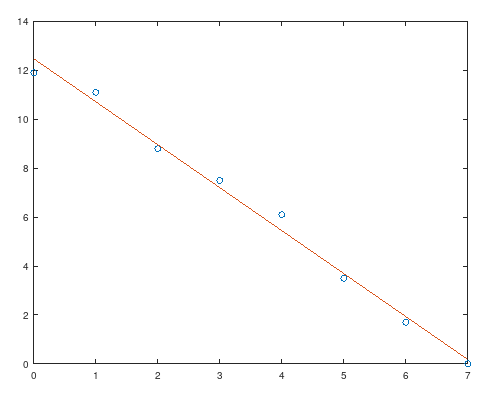
\includegraphics[scale=0.7]{pol1}
        
        Da mesma forma, inserindo $A$ e $b$ do segundo exemplo, temos:
        $$
            x =
            \begin{bmatrix}
                9.1625 \\
                -7.4685 \\
                1.1494
            \end{bmatrix}
        $$
        
        O código em \textit{octave} ficou assim:
        \begin{lstlisting}
            t = 0:7;
            t = t';
            b = [9.2; 2.8; -1.5; -2.4; -2.2; 0.3; 5.5; 13.4];
            x = [0, 0, 0];
            x(1) = input("");
            x(2) = input("");
            x(3) = input("");
            
            tt = 0:.01:7;
            p1 = x(1) + x(2)*tt + x(3)*tt.^2;
            plot(t, b, "o", tt, p1);
        \end{lstlisting}
        
        O gráfico obtido foi o seguinte: \\
        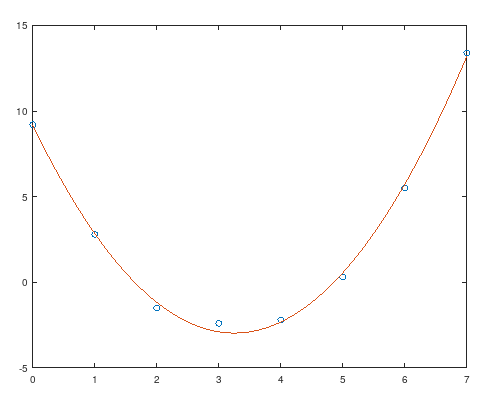
\includegraphics[scale=0.7]{pol2}
        
        Em ambos os testes a acurácia foi bem sucedida, os gráficos mostram a proximidade dos pontos dados com o polinômio estimado.
        
    \subsection{Verificando a eficiência do algoritmo}
        Para verificar a eficiência do algoritmo, utilizei as matrizes geradas aleatoriamente, aumentando $n$ e $m$ progressivamente. Medi o consumo de tempo com a subrotina \textit{cputime()} (nativa do \textit{FORTRAN}), no próprio programa. A tabela de tempos ficou assim:
        \begin{center}
            \begin{tabular}{ | c | c | c |} 
                \hline
                & & \\ [-1em]
                $n$ & $m$ & Consumo de Tempo (s)\\  [+.5em]
                \hline\hline
                & & \\ [-1em]
                20 & 10 & $4.0 \times 10^{-5}$\\ [+.5em]
                \hline
                & & \\ [-1em]
                20 & 20 & $1.3 \times 10^{-5}$\\ [+.5em]
                \hline
                & & \\ [-1em]
                200 & 100 & $8.7 \times 10^{-4}$\\ [+.5em]
                \hline
                & & \\ [-1em]
                200 & 200 & $9.3 \times 10^{-4}$\\ [+.5em]
                \hline
                & & \\ [-1em]
                2000 & 1000 & $4.9 \times 10^{-2}$\\ [+.5em]
                \hline
                & & \\ [-1em]
                2000 & 2000 & $1.1 \times 10^{-1}$\\ [+.5em]
                \hline
            \end{tabular}
        \end{center}
        Que mostra, na prática, como o algoritmo depende bem mais de $n$ em sua eficiência; afinal sempre subtraímos $\frac{2}{3}m^3$ flops da contagem de $nm^2$.
            
\end{document}

